\documentclass[10pt,a4paper,onecolumn]{article}
\usepackage{marginnote}
\usepackage{graphicx}
%\usepackage{xcolor}
\usepackage[dvipsnames]{xcolor}
\usepackage{authblk,etoolbox}
\usepackage{titlesec}
\usepackage{calc}
\usepackage{tikz}
\usepackage{hyperref}
\hypersetup{colorlinks,
            urlcolor=NavyBlue,
            linkcolor=Mulberry}
\usepackage{caption}
\usepackage{tcolorbox}
\usepackage{amssymb,amsmath}
\usepackage{ifxetex,ifluatex}
\usepackage{seqsplit}
\usepackage{enumitem}
\usepackage{xparse}
\usepackage{balance}
\usepackage{draftwatermark}
\SetWatermarkScale{1.5}
\SetWatermarkText{DRAFT}
\SetWatermarkColor[gray]{0.8}
\SetWatermarkAngle{60}

\ExplSyntaxOn

\clist_new:N \g_mapo_allauthors_clist

\NewDocumentCommand\addauthor {m}
 {
  \clist_gput_right:Nn \g_mapo_allauthors_clist { #1 }
 }

\NewDocumentCommand \printall { } { } % initialization
\DeclareExpandableDocumentCommand \printall { }
 {
  \clist_use:Nnnn \g_mapo_allauthors_clist { ~and~ } { ,~ } { ~and~ }
 }

\ExplSyntaxOff

% \usepackage{fixltx2e} % provides \textsubscript
\usepackage[backend=biber,style=apa]{biblatex}

\addbibresource{master.bib}
\addbibresource{packages.bib}

% --- Page layout -------------------------------------------------------------
\usepackage[top=3.5cm, bottom=3cm, right=1.5cm, left=1.5cm,
            headheight=2.2cm, reversemp, marginparwidth=0cm, marginparsep=0cm]{geometry}

% --- Default font ------------------------------------------------------------
% \renewcommand\familydefault{\sfdefault}

% --- Style -------------------------------------------------------------------
\renewcommand{\bibfont}{\small \sffamily}
\renewcommand{\captionfont}{\small\sffamily}
\renewcommand{\captionlabelfont}{\bfseries}

% --- Section/SubSection/SubSubSection ----------------------------------------
\titleformat{\section}
  {\normalfont\sffamily\Large\bfseries}
  {\thesection}{1em}{}
\titleformat{\subsection}
  {\normalfont\sffamily\large\bfseries}
  {\thesubsection}{1em}{}
\titleformat{\subsubsection}
  {\normalfont\sffamily\bfseries}
  {\thesubsubsection}{1em}{}
\titleformat*{\paragraph}
  {\sffamily\normalsize}


% --- Header / Footer ---------------------------------------------------------
\usepackage{fancyhdr}
\pagestyle{fancy}
\fancyhf{}
%\renewcommand{\headrulewidth}{0.50pt}
\renewcommand{\headrulewidth}{0pt}


\addauthor{{Backström, L. (202004875, LB)}}
\addauthor{{Ring, L. (202009983, LR)}}

\fancyhead[L]{\footnotesize{\sffamily \printall}.}
\fancyhead[C]{}
\fancyhead[R]{\footnotesize{\sffamily Bachelor's Project (147201E020).}}
\renewcommand{\footrulewidth}{0.25pt}

\fancyfoot[L]{\footnotesize{\sffamily Harmony in Motion: Real-time Sonification Strategies for Joint Action Research, (2023).}}


\fancyfoot[R]{\sffamily \thepage}
\makeatletter
\let\ps@plain\ps@fancy
\fancyheadoffset[L]{0cm}
\fancyfootoffset[L]{0cm}

\fancypagestyle{plain}{%
  \renewcommand{\headrulewidth}{0pt}%
  \fancyhf{}%
  \fancyfoot[L]{\footnotesize{\sffamily Harmony in Motion: Real-time Sonification Strategies for Joint Action Research, (2023).}}%
  \fancyfoot[R]{\sffamily \thepage}%
}

% --- Macros ---------

\definecolor{linky}{rgb}{0.0, 0.5, 1.0}

\newtcolorbox{repobox}
   {colback=red, colframe=red!75!black,
     boxrule=0.5pt, arc=2pt, left=6pt, right=6pt, top=3pt, bottom=3pt}

\newcommand{\ExternalLink}{%
   \tikz[x=1.2ex, y=1.2ex, baseline=-0.05ex]{%
       \begin{scope}[x=1ex, y=1ex]
           \clip (-0.1,-0.1)
               --++ (-0, 1.2)
               --++ (0.6, 0)
               --++ (0, -0.6)
               --++ (0.6, 0)
               --++ (0, -1);
           \path[draw,
               line width = 0.5,
               rounded corners=0.5]
               (0,0) rectangle (1,1);
       \end{scope}
       \path[draw, line width = 0.5] (0.5, 0.5)
           -- (1, 1);
       \path[draw, line width = 0.5] (0.6, 1)
           -- (1, 1) -- (1, 0.6);
       }
   }

% --- Title / Authors ---------------------------------------------------------
% patch \maketitle so that it doesn't center
\patchcmd{\@maketitle}{center}{flushleft}{}{}
\patchcmd{\@maketitle}{center}{flushleft}{}{}
% patch \maketitle so that the font size for the title is normal
\patchcmd{\@maketitle}{\LARGE}{\LARGE\sffamily}{}{}
% patch the patch by authblk so that the author block is flush left
\def\maketitle{{%
  \renewenvironment{tabular}[2][]
    {\begin{flushleft}}
    {\end{flushleft}}
  \AB@maketitle}}
\makeatletter
\renewcommand\AB@affilsepx{ \protect\Affilfont}
%\renewcommand\AB@affilnote[1]{{\bfseries #1}\hspace{2pt}}
\renewcommand\AB@affilnote[1]{{\bfseries #1}\hspace{3pt}}
\makeatother
\renewcommand\Authfont{\sffamily\bfseries}
\renewcommand\Affilfont{\sffamily\small\mdseries}
\setlength{\affilsep}{1em}


\ifnum 0\ifxetex 1\fi\ifluatex 1\fi=0 % if pdftex
  \usepackage[T1]{fontenc}
  \usepackage[utf8]{inputenc}

\else % if luatex or xelatex
  \ifxetex
    \usepackage{mathspec}
  \else
    \usepackage{fontspec}
  \fi
  \defaultfontfeatures{Ligatures=TeX,Scale=MatchLowercase}

\fi
% use upquote if available, for straight quotes in verbatim environments
\IfFileExists{upquote.sty}{\usepackage{upquote}}{}
% use microtype if available
\IfFileExists{microtype.sty}{%
\usepackage{microtype}
\UseMicrotypeSet[protrusion]{basicmath} % disable protrusion for tt fonts
}{}

\usepackage{hyperref}
\PassOptionsToPackage{usenames,dvipsnames}{color} % color is loaded by hyperref
\hypersetup{unicode=true,
            pdftitle={Harmony in Motion: Real-time Sonification Strategies for Joint Action Research},
            pdfkeywords={Sonification; Motion Capture; Realtime; Processing},
            colorlinks=true,
            linkcolor=Mulberry,
            citecolor=BrickRed,
            urlcolor=NavyBlue,
            }
\urlstyle{same}  % don't use monospace font for urls
\IfFileExists{parskip.sty}{%
\usepackage{parskip}
}{% else
\setlength{\parindent}{0pt}
\setlength{\parskip}{6pt plus 2pt minus 1pt}
}
\setlength{\emergencystretch}{3em}  % prevent overfull lines
\setcounter{secnumdepth}{5}
% Redefines (sub)paragraphs to behave more like sections
\ifx\paragraph\undefined\else
\let\oldparagraph\paragraph
\renewcommand{\paragraph}[1]{\oldparagraph{#1}\mbox{}}
\fi
\ifx\subparagraph\undefined\else
\let\oldsubparagraph\subparagraph
\renewcommand{\subparagraph}[1]{\oldsubparagraph{#1}\mbox{}}
\fi


% tightlist command for lists without linebreak
\providecommand{\tightlist}{%
  \setlength{\itemsep}{0pt}\setlength{\parskip}{0pt}}

% From pandoc table feature
\usepackage{longtable,booktabs,array}
\usepackage{calc} % for calculating minipage widths
% Correct order of tables after \paragraph or \subparagraph
\usepackage{etoolbox}
\makeatletter
\patchcmd\longtable{\par}{\if@noskipsec\mbox{}\fi\par}{}{}
\makeatother
% Allow footnotes in longtable head/foot
\IfFileExists{footnotehyper.sty}{\usepackage{footnotehyper}}{\usepackage{footnote}}
\makesavenoteenv{longtable}


\usepackage{booktabs}
\usepackage{longtable}
\usepackage{array}
\usepackage{multirow}
\usepackage{wrapfig}
\usepackage{float}
\usepackage{colortbl}
\usepackage{pdflscape}
\usepackage{tabu}
\usepackage{threeparttable}
\usepackage{threeparttablex}
\usepackage[normalem]{ulem}
\usepackage{makecell}
\usepackage{xcolor}

\title{Harmony in Motion: Real-time Sonification Strategies for Joint Action Research}

        \author[1]{Linus Backström}
          \author[1]{Luke Ring}
    
      \affil[1]{Aarhus University}
  \date{\vspace{-5ex}}
\begin{document}
\newgeometry{includemp, reversemp, left=1.0cm, marginparwidth=4.5cm, marginparsep=0.5cm}
    \maketitle
  % \thispagestyle{empty}% suppress header and footer on title page
      \begin{abstract}
  Placeholder: For any time-sensitive task making use of auditory feedback, having low latency is vital to ensure the sonification feels connected to the action, rather than disjointed\ldots{}
  \end{abstract}
  
  \marginpar{
    \sffamily\small
    
    {\bfseries Programme}\\BSc Cognitive Science\\[1mm]
    {\bfseries Course}\\Bachelor's Project (147201E020)\\[1mm]
    {\bfseries Supervisor}\\Anna Zamm, Assistant Professor\\[1mm]
    {\bfseries Faculty}\\Faculty of Arts\\
    Aarhus University\\[2mm]

    {\bfseries Submitted:} 4 January 2023\\[2mm]

    {\bfseries Student Details}
    \begin{itemize}[align=parleft,left=1em..2em]
      \setlength\itemsep{0em}
            \item Linus Backström\\ ID: 202004875\\ Initials: LB
            \item Luke Ring\\ ID: 202009983\\ Initials: LR
          \end{itemize}

    \vspace{2mm}

    {\bfseries Software}
    \begin{itemize}[align=parleft,left=1em..2em]
      \setlength\itemsep{0em}
      \item \href{https://github.com/zeyus/QTM\_Bela\_Sonification}{\color{NavyBlue}{Repository}} \ExternalLink
    \end{itemize}

    \vspace{2mm}

    {\bfseries License}\\
    Authors of papers retain copyright and release the work under a MIT Licence (\href{https://github.com/zeyus/QTM\_Bela\_Sonification/blob/main/LICENSE.md}{\color{NavyBlue}{MIT}}).
  }
\restoregeometry
{
\hypersetup{linkcolor=Black}
\setcounter{tocdepth}{3}
\tableofcontents
}
\twocolumn

% This will be displayed full-width
\hypertarget{harmony-in-motion-real-time-sonification-strategies-for-joint-action-research}{%
\section{Harmony in Motion: Real-time Sonification Strategies for Joint Action Research}\label{harmony-in-motion-real-time-sonification-strategies-for-joint-action-research}}

Joint action tasks form an integral part of the everyday life of humans and many other species {[}ref{]},
and the mechanisms underlying this cooperative ability to work together towards a common goal have been
the subject of an increasing number of publications {[}ref, scholar search?{]}. Many types of cooperation
involve auditory perception as a key aspect, either as the focus of the task -- as is the case for
musicians in a band -- or as a component that can be leveraged for increasing synchronization,
for example with a steady beat to set the pace for rowers. For any time-sensitive task making
use of auditory feedback, having low latency is vital to ensure the sonification feels connected
to the action, rather than disjointed {[}ref{]}. While there has been research into the effects of
sonification on joint action {[}ref{]}, this thesis presents a flexible low latency sonification
framework that uses real-time positional data for joint action research. This framework has been
implemented in a pilot study to investigate the utility of a novel joint action synchrony paradigm
that puts the focus of the sonification strategy as a core aspect of study design in this field. By
comparing subject synchronization during experiments employing task-oriented or synchronization-oriented
strategies, we have attempted to show differences that highlight the importance of strategy selection
for sonification and provide a pathway for further investigation.

\hypertarget{background}{%
\section{Background}\label{background}}

\hypertarget{joint-action}{%
\subsection{Joint Action}\label{joint-action}}

Joint actions, where two or more people synchronize their actions in pursuit of a shared goal \autocite{knoblichPsychologicalResearchJoint2011}, are a regular part of human behaviour. Examples include handshakes, conversations, musical performances, dancing\ldots{}

What are the cognitive processes involved in joint action? Recent theory suggests that the main cognitive processes involved include representations, action monitoring and action prediction \autocite{vesperMinimalArchitectureJoint2010,loehrMonitoringIndividualJoint2013,sebanzJointActionBodies2006}.

\hypertarget{representations}{%
\subsubsection{Representations}\label{representations}}

According to the minimal architecture for joint action proposed by \textcite{vesperMinimalArchitectureJoint2010}, an agent involved in joint action must, at a minimum, have a representation of their own task and the shared goal. While it is not required, it is usually helpful to also represent the other's task, as it allows for more precise predictions of what the other will do next \autocite{boltSensoryAttenuationAuditory2021}. As an example, consider two singers performing a duet together. Each singer must fully know their own part, while also representing the shared goal of synchronized singing. Although these two main representations can be sufficient for performing a duet, professional singers typically familiarize themselves with their singing partner's part in addition to their own, as it allows for a more polished and cohesive musical performance. This is supported by a study (Keller et al., 2007) where pianists were asked to record one part from a selection of piano duets and then, at a later date, play the complementary part in synchrony with either their own or other participants' recordings. The results showed that the pianists synchronized better with recordings of themselves than those of others, indicating that having more accurate representations of the other's actions facilitated synchronization.

Further insight into the role of representations in joint action comes from an EEG study by \textcite{kourtisPredictiveRepresentationOther2012}, which found that partners represented each other's actions in advance when passing an object, and doing so facilitated coordination. Having these shared representations of actions and their underlying goals allows individuals to establish a procedural common ground for joint action without needing to rely on symbolic communication \autocite{sebanzJointActionBodies2006}.

\hypertarget{action-monitoring}{%
\subsubsection{Action Monitoring}\label{action-monitoring}}

Monitoring processes are used to assess the extent to which a task or goal is being accomplished and whether actions are proceeding as intended (Botvinick et al., 2001). In terms of assessing task and goal progress, three things can be monitored: one's own task, the other's task, and the shared goal. As with representations, one must at least monitor the progress of one's own task and the shared goal. It is not strictly necessary to monitor the other's task, and it depends on the type of joint action that is performed. Nevertheless, it is likely true that monitoring what one's partner is doing will improve joint action performance -- especially for tasks that require precise synchronization \autocite{vesperMinimalArchitectureJoint2010}.

With respect to monitoring the sensory consequences or outcomes of joint actions, a distinction can be made between monitoring the individual outcomes vs joint outcomes. A study by Loehr et al.~(2013) distinguished between individual and joint outcomes of actions with the help of a clever experiment, where pianists played a pre-rehearsed duet on a digital piano while the outcomes of keypresses were manipulated by the researchers. In the individual outcome condition, the produced tones were manipulated so that the harmony of the resulting chord remained the same. In the joint outcome condition, the produced tones were manipulated so that the harmony of the chord changed. \{More text to follow, incorporating these findings: ``musicians engaged in joint actions monitor their own and their partner's actions as well as their combined action outcomes, while at the same time maintaining a distinction between their own and othersʼ actions and between individual and joint outcomes.{[}\ldots{]} The first goal of the current study was to provide further evidence that people monitor their own and their partnersʼ action outcomes in parallel. The second goal of the current study was to investigate whether people monitor each personʼs individual part in a joint action and/or the combined outcome of their coordinated actions. {[}\ldots{]} These findings indicate that skilled performers are able to monitor the outcomes of their own actions, their coperformersʼ actions, and their combined actions when they perform joint actions together. They also indicate that performers nevertheless differentiate between their own and othersʼ action outcomes and between individual and joint action outcomes.``\}

\hypertarget{action-predicting}{%
\subsubsection{Action Predicting}\label{action-predicting}}

In order to coordinate effectively, it is often necessary to make predictions about future events. This prediction process is achieved through motor simulation, which uses internal models to determine the sensory consequences of actions as well as their effect on the environment (Gerd Schmitz \& Alfred O. Effenberg, 2017; Vesper et al., 2010). Simulating the actions of others as they occur may be especially beneficial when engaging in joint action, as it is believed to influence perception and assist in predicting the consequences and timing of others' actions (Vesper et al., 2010). The idea that internal predictive models contribute to the ability to anticipate others' actions is supported by findings that short-term predictions of others' actions are based on one's own motor experience (Aglioti et al., 2008; Calvo-Merino et al., 2005). It is not fully clear yet whether similar mechanisms exist specifically for predicting the joint outcome of an agent and their partner. Some support for predicting joint outcomes comes from a study by Knoblich \& Jordan (2003) which demonstrated the ability to predict combined outcomes through improved joint task performance with practice. The results showed that participants initially struggled with the joint task of controlling a cursor together to track a moving target on a computer screen, but with practice, performance reached the level of individual performance.

\hypertarget{integrating-predicted-outcomes-of-ones-own-and-others-actions}{%
\subsubsection{Integrating Predicted Outcomes of One's Own and Others' Actions}\label{integrating-predicted-outcomes-of-ones-own-and-others-actions}}

The crucial final feature of joint action is the manner in which individuals adapt their own actions to those of others in time and space. The question concerns the decision-making process that occurs after a prediction of another person's action is made, i.e.~choosing a suitable complementary action and performing it at the appropriate time. In order to avoid constantly being one step behind during joint action, interacting partners cannot simply respond to observed actions, but must rather plan their own actions in relation to what they predict their partner will do \autocite{sebanzJointActionBodies2006}. A study by Knoblich and Jordan {[}Sebanz 43-34{]} using a joint action tracking paradigm found that partners planned their actions based on a prediction of what the joint effect of both their own and their partner's actions would be.

Some of the questions that have been investigated in recent joint action research concern the aforementioned processes (representations, action monitoring and action predicting) and how they relate to agency (self vs other) and outcome (individual vs joint). Researchers have studied whether agents involved in joint action represent both their own task and their partner's task (citation), whether they monitor individual outcomes or joint outcomes, and\ldots{} The current study primed the participants' attention towards individual and joint outcomes in different conditions while investigating joint task synchronization.

\hypertarget{current-study}{%
\subsubsection{Current Study}\label{current-study}}

The current study had participants perform a joint action task under three different conditions, where the sensory consequences were manipulated through real-time sonification of movement.

The current study focuses on what happens during learning of joint action. Through movement sonification, we can enhance attention towards specific features of joint action. Is learning optimized when focusing on self-other representations or joint outcome representations?

While we could not completely separate the conditions, our sonification primes attention towards either self-other monitoring, or joint outcome.

\hypertarget{sonification}{%
\subsection{Sonification}\label{sonification}}

Sonification is defined as the use of nonspeech audio to convey information. More specifically, sonification is the transformation of data relations into perceived relations in an acoustic signal for the purposes of facilitating communication or interpretation \autocite[p.~4]{kramerSonificationReportStatus1999}.

While concepts around sonification and audification were not formalized until around the year 1992 when the first International Conference on Auditory Display (ICAD) was held \autocite{dubusSonificationPhysicalQuantities2011}, practical examples of sonification can be found throughout history. Water clocks in ancient Greece and medieval China were sometimes constructed to produce sounds and thereby provide auditory information about the passage of time \autocite{dubusSonificationPhysicalQuantities2011}. The stethoscope, which is used for listening to sounds made by the heart and lungs as well as other internal sounds of the body, was invented in 1816 by French physician and amateur musician Rene Laënnec \autocite{roguinReneTheophileHyacinthe2006}. The Geiger counter developed in 1928 provides perhaps the most characteristic example of sonification through its function of sonifying levels of radiation. The device detects ionizing radiation and translates it into audible clicks, where a faster tempo signifies a higher level of radiation. \textcite{dubusSonificationPhysicalQuantities2011} describe the value of the Geiger counter as ``transposing a physical quantity which is essentially non-visual and pictured in everyone's imagination as very important because life-threatening, to the auditory modality through clicks with a varying pulse''.

\hypertarget{what-is-sonification-useful-for}{%
\subsubsection{What is sonification useful for?}\label{what-is-sonification-useful-for}}

\{this section is just raw, copypasted quotes for now\}
Making sense of large amounts of data, and utilizing modern powerful media technologies. ``Sonification research is well positioned to provide technology to assist scientists in comprehending the information and data-rich world of today and of the future.''. ``The wide availability of audio technology (e.g., in multimedia computers) makes auditory data representation a viable option for large numbers of users. Thus, there exists today a synergism between the widespread need for new data comprehension methods and readily available technology that, with proper support and funding, can lead to a large number of users reaping the benefits conferred by the development of scientific sonification.'' \autocite{kramerSonificationReportStatus1999}

\hypertarget{movement-sonification}{%
\subsubsection{Movement sonification}\label{movement-sonification}}

\{this section is just raw, copypasted quotes for now\}
``Approaches within the discipline of Sport Science reflect the whole range from fundamental research with high internal validity to applied research with high ecological validity. Applied research plays an important role for the development of new, more effective intervention methods. Assuming that more senses are more powerful in perceiving gross motor patterns it should be supportive to create and convey more acoustic movement information. For multisensory integration benefits, additional auditory movement information has to correspond to the structure of a perceptual feature stream of another modality (visual, kinesthetic, tactile). For such an acoustic enhancement of motor perception Effenberg (1996, 2004, 2005) has established the concept of `movement sonification', adapting the sonification approach of the early 1990s to the kinematics and dynamics of human motor behavior.'' One of the movement parameters that can be used is ``kinematic parameters representing the spatiotemporal features of a pose or a movement pattern.'' ``The question whether dynamic or kinematic movement parameters should be chosen for movement sonification should be answered under consideration of the sensory modality or modalities with which bi- or multimodal convergence should be achieved: If visual motion perception is the reference, movement sonification should be based on kinematic parameters.'' \autocite{gerdschmitzSoundJoinedActions2017}

\begin{quote}
``Subjects are able to perceive differences in swimming stroke frequency more accurately when visualizations of a swimmer are complemented with a kinematic sonification.'' \autocite{gerdschmitzSoundJoinedActions2017}
\end{quote}

\hypertarget{auditory-perception}{%
\subsubsection{Auditory perception}\label{auditory-perception}}

Research into auditory perception indicates two basic features of auditory perception that provide good arguments for representing data as sound. First, auditory perception is especially useful for detecting temporal characteristics, i.e.~variations in sound over time. {[}find study that said we're better at detecting rhythm aurally vs visually?{]} Sonification can thus be useful for monitoring or understanding complex temporal data. Second, our sense of hearing does not require us to be oriented towards the sound source. Unlike visual perception, which allows us to perceive approximately 180 degrees of our environment in front of us while we remain blind to the other 180 degrees behind us, auditory perception allows perception of 360 degrees. This makes auditory signals particularly useful for situations where our visual system is occupied with another task and we cannot afford to look around constantly, such as monitoring and alarm applications. \autocite{kramerSonificationReportStatus1999}

Other benefits of auditory perception that speak for sonification: parallel listening (ability to monitor and process multiple auditory data sets), rapid detection (especially in high-stress environments), affective response (ease of learning and high engagement qualities) and auditory gestalt formation (discerning relationships or trends in data streams) \autocite{kramerSonificationReportStatus1999}.

\hypertarget{hardware-and-software-implementation}{%
\section{Hardware and Software Implementation}\label{hardware-and-software-implementation}}

\hypertarget{motion-capture}{%
\subsection{Motion Capture}\label{motion-capture}}

Motion capture data were collected using a 9 camera (8 Qualisys Miqus M3 marker and 1 Qualisys Miqus Video) system connected to a Qualisys Camera Sync Unit.
Marker data were acquired at a sampling rate of 300 Hz and video data were acquired at a sampling rate of 25 Hz. Qualisys Track Manager version 2022.2 (build 7700) software was used to collect and process the data with real-time 3D tracking data output.

\hypertarget{markers}{%
\subsubsection{Markers}\label{markers}}

For the experimental set up, one passive marker was placed on each car, and two additional passive reference markers were placed on the front corners of the track (see Fig X). These additional markers provided reference points for 3D orientation of the track and the cars across trials in case of accidental track movement. QTM Automatic Identification of Marker (AIM) models were trained on variable speed sled movements along the track and were given labels for client-side identification.

\hypertarget{event-labels}{%
\subsubsection{Event Labels}\label{event-labels}}

Event labels were sent to QTM to mark the start and end of each condition and each trial within that condition.

\hypertarget{sonification-1}{%
\subsection{Sonification}\label{sonification-1}}

Motion capture data were sent via UDP packets over USB networking to a Bela Mini device running version 0.3.8g running a custom C++ program\footnote{Source, data and analyses are available at \url{https://github.com/zeyus/QTM_Bela_Sonification}}. The main program loop was configured to execute every 32 samples, with an output sample rate of \ensuremath{4.41\times 10^{4}} Hz for 2 audio channels. The two audio output channels were connected to a pair of Genelec G Two active speakers. The main program used the Bela platform framework from 10 August 2022\footnote{\url{https://github.com/BelaPlatform/Bela/commit/42bbf18c3710ed82cdf24b09ab72ac2239bf148e}}. The experiment flow control was automated using the defined time periods for trials and breaks between them, and paused between conditions until a button on the device was pressed to allow sufficient time for subjects to rest and answer the IOS survey. Figure {[}xxx{]} describes the flow of data from motion capture to sonification.

\hypertarget{real-time-3d-data}{%
\subsubsection{Real-time 3D Data}\label{real-time-3d-data}}

A version of the Qualisys C++ SDK using protocol version 1.23 was modified to be compatible with the Bela platform and was used for communicating with QTM. To reduce latency, connection to the QTM server was made over UDP, and round-trip communication latency was verified by performing 1000 requests to the server and logging the elapsed time between resulting in a mean latency of x.xxxms (sd/min/max).
Using the SDK, 3D streaming was initiated at the start of each sonification condition, and labelled markers were used to obtain the current position of each sled. The coordinates of the sleds were stored in a buffer containing the current and last recorded coordinates.

\hypertarget{methods}{%
\section{Methods}\label{methods}}

\hypertarget{pilot-experiment}{%
\subsection{Pilot Experiment}\label{pilot-experiment}}

A pilot experiment was conducted to assess the viability of the sonification framework in a laboratory setting. This experiment required blindfolded subjects to move their assigned sleds along parallel tracks and use sounds they hear to remain as spatially synchronized as possible.

\hypertarget{participants}{%
\subsection{Participants}\label{participants}}

An availability sample of ten subjects were recruited to participate in pairs, subjects were all aged between 20 and 30 years and were a mix of genders and handedness. Most subjects also reported no formal musicianship training. (prioritized comfort, allowed choice of arm despite handedness) {[}why this many, why not more, etc, ethics{]} Subjects were given and signed an informed consent form and information sheet and were under the umbrella project\ldots{}

\hypertarget{experimental-design}{%
\subsection{Experimental Design}\label{experimental-design}}

Participants were asked to sit on opposite sides of the track structure and familiarize themselves with the movement of the sleds along the tracks. They were instructed to try to continuously move the sleds back and forth along the track as rapidly as possible while remaining spatially synchronized with their partner's position on their respective track, using sounds they may hear during the various conditions to assist them. After the conclusion of subject briefing and they had indicated they were ready, they were blindfolded for the duration of all trials within a condition, with a pause between conditions where they could rest and remove the blindfold.

\hypertarget{track-and-sleds}{%
\subsubsection{Track and Sleds}\label{track-and-sleds}}

Two parallel tracks were designed with a sigmoid curve shape, surfaced with a smooth veneer that allowed for free movement along the length of the track. Two identical sleds made from LEGO parts were constructed and three felt adhesive pads were attached to the underside of each to reduce resistance during movement. See Figure \ref{fig:track-setup}

\begin{figure}

{\centering 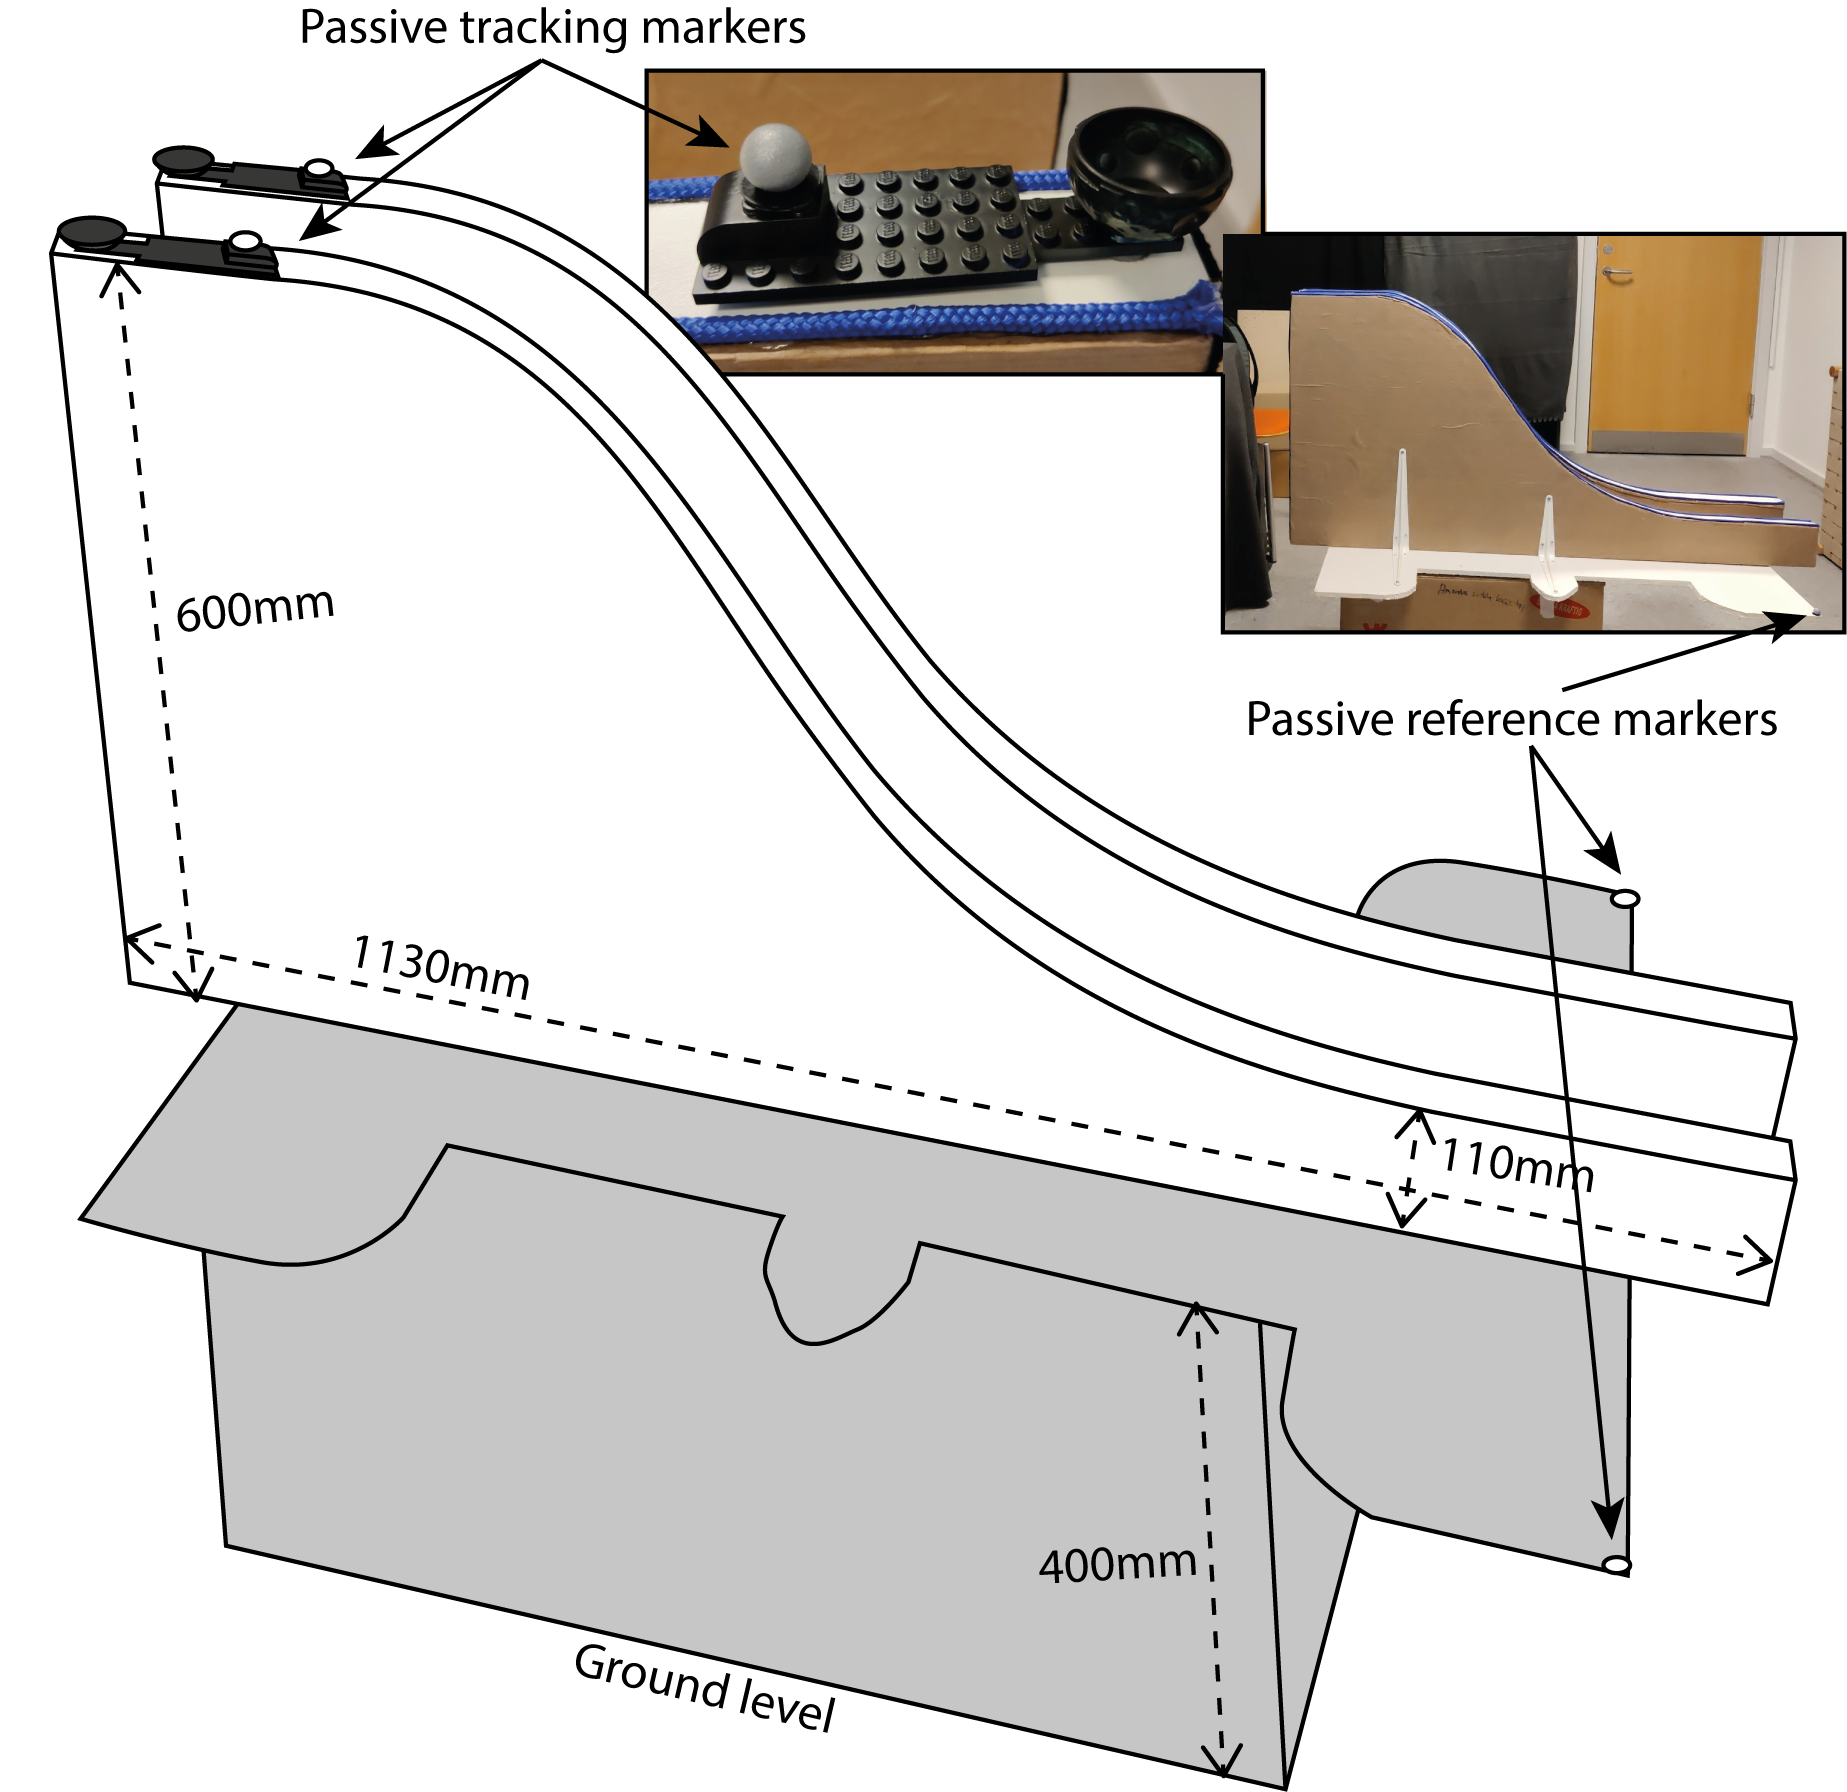
\includegraphics[width=1\linewidth]{figures/track_dimensions} 

}

\caption{Experimental track setup showing track shape and dimensions}\label{fig:track-setup}
\end{figure}

\hypertarget{frequency-range-selection}{%
\subsubsection{Frequency Range Selection}\label{frequency-range-selection}}

Two distinct, continuous frequency ranges were selected for application in sonification conditions. These ranges are offset by a perfect fifth and span eight semitones, the overtone range was chosen based on a center frequency of 440Hz (A4) and the range was limited to avoid a large overlap with the undertone range during normal operation (Table X). Consideration was also given to creating ranges that were not sufficiently high to cause discomfort, nor sufficiently low that distinguishing slight differences becomes more difficult.

\begin{table}

\caption{\label{tab:frequency-ranges}Frequency ranges for the two tones used in the sonification conditions. Note names are in International Pitch Notation, and are the closest approximation. Overtone frequencies were calculated to have a center frequency of 440Hz, and undertone frequencies are two-thirds of their overtone counterparts.}
\centering
\fontsize{7}{9}\selectfont
\begin{tabular}[t]{llrcrcr}
\toprule
\multicolumn{1}{c}{} & \multicolumn{2}{c}{Lower Bound} & \multicolumn{2}{c}{Center} & \multicolumn{2}{c}{Upper Bound} \\
\cmidrule(l{3pt}r{3pt}){2-3} \cmidrule(l{3pt}r{3pt}){4-5} \cmidrule(l{3pt}r{3pt}){6-7}
  & Freq & Note & Freq & Note & Freq & Note\\
\midrule
Overtone & 349.230 & F4 & 440.000 & A4 & 554.365 & C\#5\\
Undertone & 232.819 & A\#3 & 293.333 & D4 & 369.577 & F\#4\\
\bottomrule
\end{tabular}
\end{table}

Table X: Note names are in International Pitch Notation, and are the closest approximation. Overtone frequencies were calculated to have a center frequency of 440Hz, and undertone frequencies are two-thirds of their overtone counterparts.

\hypertarget{sonification-strategies}{%
\subsubsection{Sonification Strategies}\label{sonification-strategies}}

The experiment consisted of three conditions that vary the sonification strategy employed, namely: a no sonification control condition, a task-oriented sonification strategy and a synchronization-oriented sonification strategy. Each condition consisted of one practice trial of 30 seconds duration, and three main trials of 90 seconds each. Before each practice trial, subjects were reminded that it was a shorter trial and that they may use it to experiment with the sonification.

\hypertarget{no-sonification.}{%
\paragraph{No sonification.}\label{no-sonification.}}

In the no sonification condition, only the motion capture data were recorded, and subjects could use the audible sounds of the sleds moving along the track to align themselves with their partner.

\hypertarget{task-oriented-sonification-strategy.}{%
\paragraph{Task-oriented sonification strategy.}\label{task-oriented-sonification-strategy.}}

Task oriented sonification represented the position of each sled along the length of the track as a synthesized tone that varied in frequency from highest to lowest at the start and end of the track respectively. One sled produced a higher frequency overtone, while the other produced a lower frequency undertone. If subjects were at the exact same y-coordinate, the two tones would be a perfect fifth apart, creating a harmonious chord, as the sleds drift further apart, the frequency difference would deviate from the perfect fifth and create a more discordant sound. This strategy was selected for sonifying the movement along the track, i.e.~the task required of subjects.

{[}Figure here illustrating task sonification{]}

\hypertarget{synchronization-oriented-sonification-strategy.}{%
\paragraph{Synchronization-oriented sonification strategy.}\label{synchronization-oriented-sonification-strategy.}}

The sonification strategy oriented around synchronization represented the position of the sleds relative to each other,\ldots{}

\hypertarget{procedure}{%
\subsection{Procedure}\label{procedure}}

This is where the experiment flow will be described.

\hypertarget{data-analysis}{%
\section{Data Analysis}\label{data-analysis}}

{[}General timing stuff, project specific stuff.{]}

\hypertarget{data-preprocessing}{%
\subsection{Data Preprocessing}\label{data-preprocessing}}

\hypertarget{qtm}{%
\subsubsection{QTM}\label{qtm}}

Each session recorded had the AIM model applied to the duration of the recording, and labelled markers were manually verified and adjusted as required to ensure that for each completed trial, there was 100\% coverage of the marker data. Processing of every frame and 2D data preprocessing were disabled for real-time output to ensure minimal latency.

\hypertarget{results}{%
\section{Results}\label{results}}

{[}Describe{]}

\hypertarget{discussion}{%
\section{Discussion}\label{discussion}}

{[}Explain{]}

How might our task be affected by musical training? ``Successful music performance requires that musicians monitor the auditory consequences of their actions. Years of training on an instrument lead to strong associations between a given movement or set of movements and a given auditory outcome.'' (Loehr et al., 2013)

Mention the marker placement as being problematic. Also the number of reference markers\ldots also that we wanted to use headphones\ldots{}

• How does our task compare to e.g.~Loehr et al.~piano duet task?
• What can and can't our task reveal?
o Can't say that only one of the participants makes a mistake, since the goal is to in sync with each other, without a general ``tempo'' to follow
• Individual representations vs joint outcome representations?
o Often can't mirror the other person exactly

\begin{figure}

{\centering 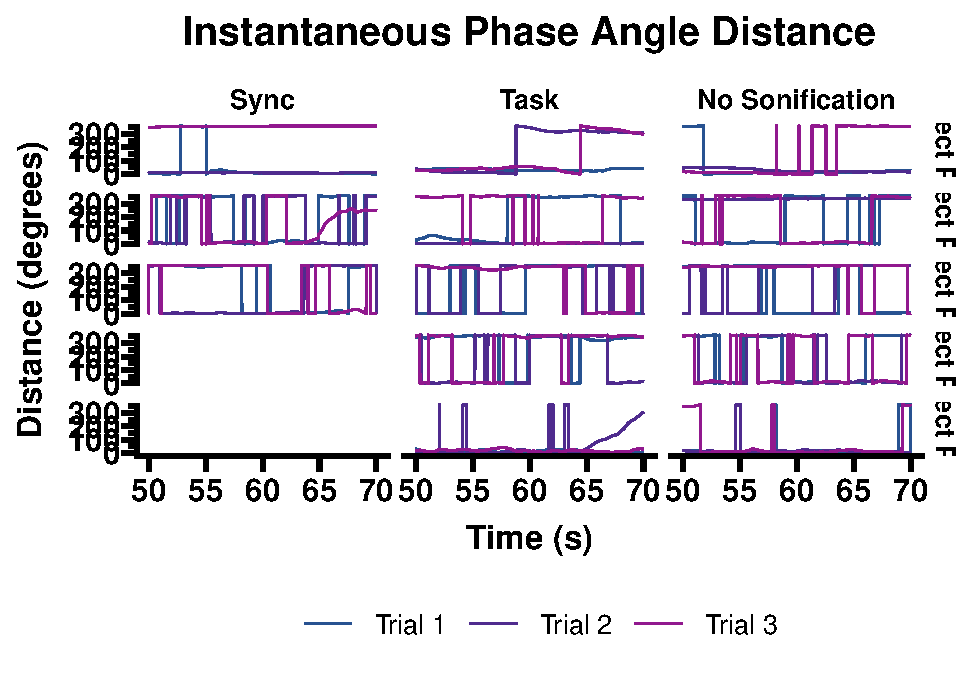
\includegraphics[width=1\linewidth]{CogSci_Bachelor_Thesis_files/figure-latex/mean-pairwise-phase-angles-1} 

}

\caption{Plot of mean pairwise phase angles for each subject pair}\label{fig:mean-pairwise-phase-angles}
\end{figure}

\begin{figure}

{\centering 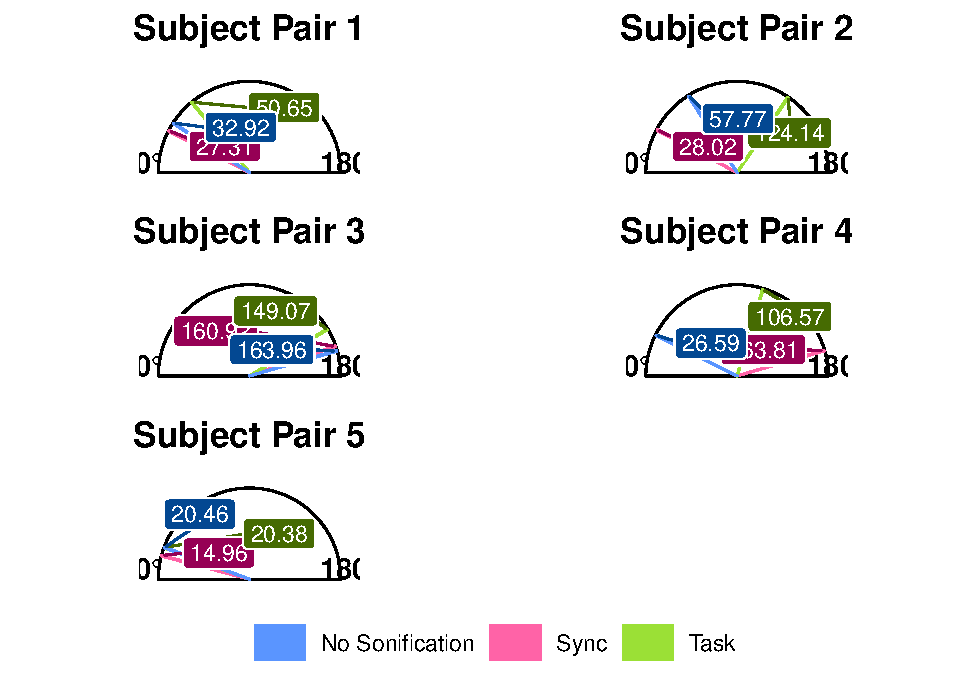
\includegraphics[width=1\linewidth]{CogSci_Bachelor_Thesis_files/figure-latex/instantaneous-phase-angle-circular-plot-1} 

}

\caption{Plot of mean pairwise phase angles for each subject pair}\label{fig:instantaneous-phase-angle-circular-plot}
\end{figure}

\hypertarget{results-1}{%
\section{Results}\label{results-1}}
\balance
\clearpage


\printbibliography[title=References,heading=bibintoc]

\end{document}
